\documentclass[10pt]{article}
\usepackage{graphicx}
\usepackage[spanish]{babel}
\usepackage{amsmath}
\usepackage{amssymb}
\usepackage{subfigure}

\begin{document}
\title{Tarea1}
\author{Mauricio Yamil Tame Soria}
\maketitle

\begin{abstract}
Se eval\'uan 1000 puntos en una funci\'on para calcular la derivada 
num\'ericamente usando la f\'ormula de diferencias finitas. Las 
operaciones fueron realizadas con un programa escrito en fortran90 y el 
texto escrito en LaTex.
\end{abstract}

Palabras clave: Fortran90, LaTex, Diferencias finitas

\section{Introducci\'on}
La tarea1 consiste en un programa que eval\'ua 1000 puntos de una funci\'on para despu\'es obtener su derivada en 999 puntos mediante la 
f\'ormula de diferencias finitas. La finalidad de la tarea es aprender a usar las herramientas de c\'omputo necesarias para la materia, Fortran90 
y LaTex.

\section{Materiales y M\'etodos}
\subsection{Programa}
El programa est\'a� estructurado en 4 archivos, dos m\'odulos, un conjunto de subrutinas y un programa principal que las llama. Los m\'odulos son un 
conjunto de variables y otro de par\'ametros, en el m\'odulo de par\'ametros est\'a $n$ que es el n\'umero de puntos que se 
eval\'uan y est\'an las cotas que definen el intervalo donde se evaluar\'a la funci\'on. En el m\'odulo de variables hay tres vectores de 
tama~no $n$, el vector $F$ que corresponde a los valores de la funci\'on, el vector $X$ que contiene los valores donde se evaluar\'a la 
funci\'on y 
el vector $D$ donde se almacenan los valores obtenidos para la derivada. Las subrutinas son 3, una 
para asignar memoria a los vectores que son de memoria din\'amica e inicializar los valores de los vectores $X$ y $F$, otra subrutina es para 
efectuar el c\'alculo de la derivada y almacenar los datos en el vector $D$, finalmente la \'ultima subrutina es para escribir los datos obtenidos 
en un archivo de texto para despu\'es graficar los resultados en un formato .png usando Gnuplot. Dentro del programa principal solamente 
se llaman las subrutinas para la obtenci\'on de los datos.

\subsection{Metodolog\'ia}
El intervalo escogido fue de 0 a $2\pi$ para evaluar la funci\'on $cos(x)$. Primero se calcul\'o el valor de los pasos en $x$ con la 
siguiente f\'ormula.

\begin{equation}
	\Delta x= \frac{C_s - C_i}{n}
	\label{name}
\end{equation} 

donde $C_s$ es la cota superior y $C_i$ cota inferior. Una vez obtenido ese valor se procede a hacer la discretizaci\'on del intervalo iterando de 0 
a $n$ y llenando el 
vector $X$ con la 
condici\'on 
$X(i)=i \Delta x$. Una vez que tenemos el intervalo discretizado hacemos la evaluaci\'on de la funci\'on en cada punto con otra 
iteraci\'on de 0 a $n$ haciendo $F(i)=cos(X(i))$. Ya que tenemos el intervalo discretizado y los puntos evaluados con la funci\'on podemos calcular 
la derivada de la funci\'on usando la f\'ormula de las diferencias finitas

\begin{equation}
	f'(x)=\frac{f(x+\Delta x)-f(x)}{\Delta x}
	\label{name2}
\end{equation}

usando la ecuaci\'on (\ref{name2}) llenamos el vector $D$ haciendo $D(i)=\frac{F(i+1)-F(i)}{\Delta x}$ obteniendo los valores de la derivada en los 
$n-1$ puntos. Cuando los vectores 
han sido llenados guardamos los valores en archivos de texto para graficar los datos con Gnuplot usando el formato png que ofrece.

\section{Resultados}
Se obtienen dos gr\'aficos, uno representa la funci\'on que se evalu\'o y el otro es su derivada. 

\begin{figure}[h]
	\centering
	\begin{minipage}{.4\textwidth}
		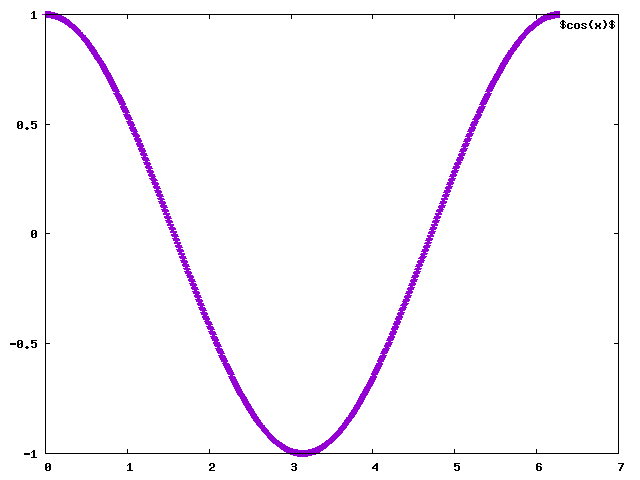
\includegraphics[width=\textwidth]{cos.png}
		\caption{coseno evaluado en 1000 puntos entre 0 y $2\pi$}
	\end{minipage}
	\hfill
	\begin{minipage}{.4\textwidth}
		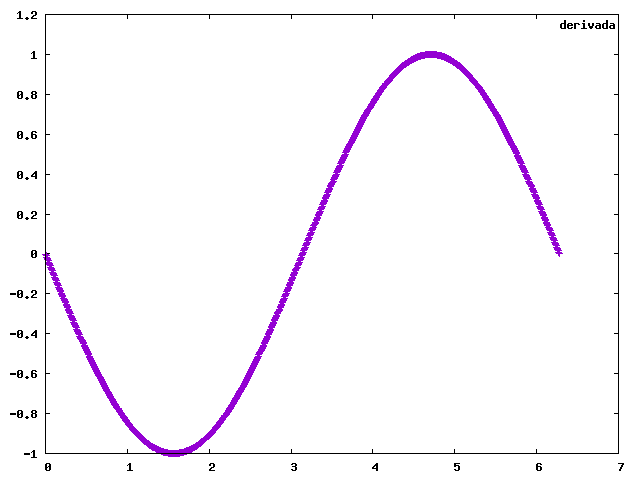
\includegraphics[width=\textwidth]{derivada.png}
		\caption{derivada de la funci\'on}
	\end{minipage}
\end{figure}

\section{Discusi\'on}
Los resultados obtenidos son los esperados, la gr\'afica de la derivada claramente representa un $sen(x)$ que es la derivada anal\'itica de la 
funci\'on coseno. Ser\'ia interesante calcular el error que tienen los valores obtenidos con el m\'etodo y los valores anal\'iticos, podr\'iamos 
usar la ecuaci\'on 

\begin{equation}
Error=|f'_n - f'_a|
\end{equation}

donde $f'_m$ es el valor obtenido por el m\'etodo y $f'_a$ es el valor anal\'itico, posiblemente en futuras pr\'acticas utilicemos esta herramineta 
de an\'alisis.

\section{Conclusiones}
El m\'etodo num\'erico para obtener la derivada de una funci\'on es fiable, podr\'iamos hacer m\'as exacta la aproximaci\'on incrementando $n$ para 
que al usar la equaci\'on (\ref{name}) obtengamos un intervalo con m\'as puntos que se traduce a una mayor definici\'on de nuestra malla.

\end{document}
